\documentclass{article}

%opening
\title{Predicting the Helpfulness of Customer Reviews}
\author{Alex Hankin, Charlie Perkins, Sam Schick}
\date{}
\usepackage{multicol, caption, graphicx}
\usepackage[margin=1in]{geometry}
\newenvironment{Figure}
	{\par\medskip\noindent}
	{\par\medskip}
\graphicspath{{images/}}
\setlength\columnsep{20pt}
\usepackage[bottom]{footmisc}
\begin{document}

\maketitle

\begin{abstract}
	Online shopping is becoming the standard way to buy a product. As this shift occurs, it becomes more difficult to examine a product personally, and we rely more on reviews submitted by other customers. However, these reviews can be very mixed in quality. Amazon crowdsources the determination of which reviews are helpful by allowing customers to mark which reviews they found most useful, but makes no attempt to determine whether a newly submitted review is of reasonable quality. We present a system that uses the random forest algorithm to examine the text of a review and predict how helpful it will be, based on data collected from Amazon's crowdsourced data.
\end{abstract}
\begin{multicols}{2}
\section{Introduction}
	Many online reviews will never be marked helpful. However, when first published these reviews are put on equal footing with reviews that could nominally be very well written. A system that could sort these by how helpful they are likely to be found could improve customer outcomes by making it easier for them to find a wide variety of helpful reviews. For a prototype system, we gathered data from Amazon reviews on popular books, which have many reviews and also tend to have a somewhat standard format. We implement a random forest classifier that examines normalized word frequencies and attempts to predict whether the book will be in the top 90\% in terms of helpfulness. 

\section{Data Sources}

We decided that the most valuable review data would come from the most popular books, as they would have the highest number of reviews along with the greatest amount of people who decided to rank helpfulness. The 11 books selected were Dune, Harry Potter and the Prisoner of Azkaban, A Game of Thrones, the Hobbit and the Lord of the Rings Trilogy, Nineteen Eighty-Four, A Tale of Two Cities, the Road, Pride and Prejudice, the Giver, the Catcher in the Rye, and the Great Gatsby. For each one, we gathered the top 40 to 100 reviews, as ranked by Amazon, along with the number of people who marked each review helpful. Ultimately, the goal was to gather most of the reviews that at least one person ranked. Data was taken using the Scrapy framework. Scrapy offers a simple method for taking data from websites that appears in the html code. After indicating the webpage and the associated html excerpts we want to scrape, our program saves each review and helpfulness rank into a dat file, which may then be used for post-processing and analysis.


\section{Text Processing}

The main issue that we foresaw when scanning through various different book reviews, was coming across words that would be unique to the book being reviewed. Most of the time these would consist of proper nouns, such as names of characters, book titles, and other unique items limited to that one book. We decided that the mentioning of these specific words was not important, but rather the quality and description of the books themselves being discussed around the proper nouns. Thus, we wanted to remove the proper noun variable entirely. To do this we used the Natural Language Toolkit (NLTK) in a file that takes in any given review and uses the tagging function to determine whether or not a word in the review is a proper noun. If a word is a proper noun, we replace it with the keyword “Proper\_Noun"; this allowed the classifier to treat the group of proper nouns as a single feature. 
 
This method was not without its limitations, for one, the NLTK’s algorithm that detects proper nouns simply checks if the first letter is uppercase, and then instantly tags it as proper. This causes a few problems; for example, when a casual reviewer chooses not to capitalize their proper nouns, or common words that still begin with an uppercase letter such as those at the beginning of a sentence. The programming compromise was to have NLTK ignore words that began a sentence, and then compile all proper nouns found elsewhere into a list. Then create a copy of that list that contains lower case variations, and search the entire review for instances of these words and replace them with our keyword if they are found. This means the only time a proper noun is ignored is if an instance is always lowercase in the review, or if it is only ever seen at the beginning of a sentence. This method will also never incorrectly assume a common word is a proper noun. With this optimized to the best of NLTK’s ability we converted all of our reviews to an easy to analyze format.

\section{Feature Extraction and Regression}

In examining counts of helpfulness, we ran into a variety of confounding factors. The first is that when a review is marked helpful, it is shown first in the ordering. This makes it more likely to be marked helpful again. Because of this, independent of the actual helpfulness of the reviews, the helpfulness ratings tend to follow an exponential curve. To compensate, before further examining helpfulness scores we took their log value to create a more linear data set. In addition, the number of helpful marks varies widely from book to book, with more popular books being marked more helpful. We normalized each book separately, with the most helpful review for each book normalized to a score of 1. We then combined these lists into a master list, and took our class of "bad" reviews to be the bottom 10\% of this list.

We used the bag of words methodology to extract features. We represented each document as a vector, where each entry was a word that occurred in the document and had value equal to the number of times the word occurred in that document. This gave us a matrix where each row was a word and each column was a review. We normalized this data using TFIDF (Term Frequency Inverse Document Frequency). This allows soft filtering of low value words by scaling down words which occur very frequently across the data set. We then used the random forest algorithm as implemented by SKLearn to create a classifier. Random forest generates decision trees based off of a random subset of features (in this case, words). Each decision tree produces a regression, and these predictions are combined to reduce variance in the output. each review was considered "bad" if it was in the bottom 10\% in terms of helpfulness for the book it had come from, and "good" otherwise. The threshold was arbitrary, but this allowed us to improve the quality of the model by reducing it to a classification problem. This remains useful as a potential tool, as comments marked by the automated filter to be unhelpful could be listed last, improving user experience.

\section{Performance Evaluation}

We used stratified 3 fold cross validation to examine the quality of the model to avoid bias from the training set, separating the data out into 3 subsets each of which had shares of good and bad reviews approximately representative of the whole data set. We then built 3 versions of the model. Each model was built on 2 of the folds as a training set and the remaining fold as the tuning set. We then generated ROC curves and F1 score (harmonic mean of precision and recall) for each fold. We used these statistics to iteratively improve the structure of the classifier until we arrived on the model presented here.

\section{Analysis and Conclusions}
The average F1 score over the 3 folds was .95, which suggested a very high quality classification. The ROC curves below similarly suggest a robust classifier. However, for a product that could be implemented, much progress is still needed.
\begin{Figure}
	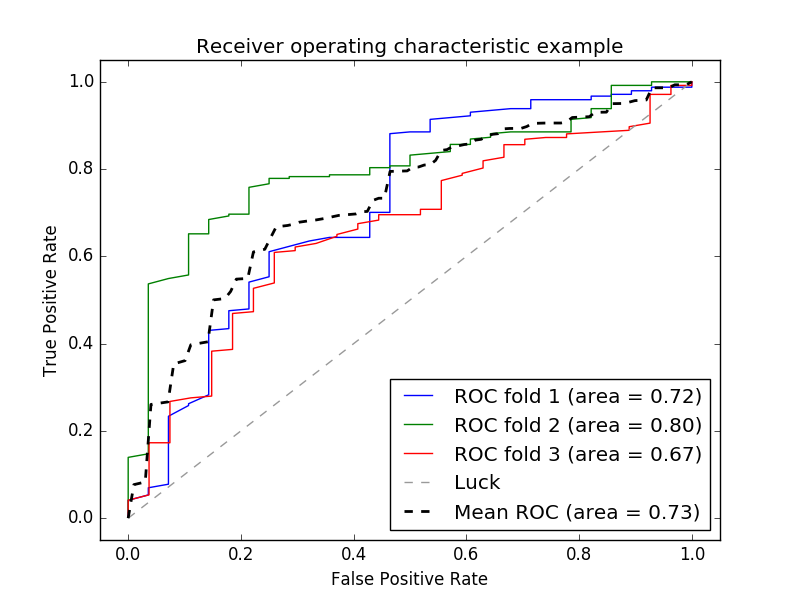
\includegraphics[width=0.5\textwidth]{ROC}
	\captionof{figure}{ROC curves generated using Scikit-Learn.}
\end{Figure}

There are a variety of ways these results could potentially be improved. The first and most obvious is scaling; the work we present here works off a relatively small set of data. In addition, due to problems in the html containing the reviews we were unable to access reviews with 0 marks of helpful, leading to a somewhat biased data set for training. Stronger negative examples could significantly improve the quality of the classification. Metadata about reviews could also be very useful; for example, in order to accurately examine the helpful count it should be weighted by how recently the review was posted, and a review from someone who publishes a hundred high quality reviews a year is a priori more likely to be of high quality than a review submitted from a new user. However, without more development time our methods were unable to access such metadata. Further work in the area should focus on integrating such data into a text classification to improve predictions.
\end{multicols}

\begin{thebibliography}{9}
	\bibitem{scikit} \textit{Scikit-learn: Machine Learning in Python}. Pedregosa et al.
	
	\bibitem{forests} Leo Breiman and E. Schapire. \textit{Random Forests}. Machine Learning, 2001, pg. 5-32.
	
	\bibitem{nltk} Bird, Steven, Edward Loper and Ewan Klein (2009), Natural Language Processing with Python. O’Reilly Media Inc.
\end{thebibliography}
\end{document}
